%!TEX program = xelatex
%# -*- coding: utf-8 -*-
%!TEX encoding = UTF-8 Unicode

\documentclass{beamer}
%
% Choose how your presentation looks.
%
% For more themes, color themes and font themes, see:
% http://deic.uab.es/~iblanes/beamer_gallery/index_by_theme.html
%

\mode<presentation>
{
  \usetheme{default}      % or try Darmstadt, Madrid, Warsaw, ...
  \usecolortheme{default} % or try albatross, beaver, crane, ...
  \usefonttheme[onlymath]{serif}  % or try serif, structurebold, ...
  \setbeamertemplate{navigation symbols}{}
  \setbeamertemplate{caption}[numbered]
}

\usepackage{multirow}
\usepackage{array, booktabs}
\usepackage{threeparttable}
\usepackage{dcolumn}

\usepackage{fontspec}
\setsansfont{Myriad Pro}

\usepackage[final]{microtype}

\usepackage{graphics}
\usepackage{graphicx}
\usepackage{subcaption}

\usepackage{color}
\usepackage{soul}
\usepackage{pifont}
\newcommand{\cmark}{\ding{51}}
\newcommand{\xmark}{\ding{55}}

\usepackage{fancyvrb}
\fvset{fontsize=\scriptsize}
\RecustomVerbatimEnvironment{verbatim}{Verbatim}{}


\linespread{1.3}

\title{Learning to Classify PC Malwares}
\author{Jingxiang Li \and Advisor: Yuhong Yang}
\institute{School of Statistics, UMN}
\date

\begin{document}

\begin{frame}
  \titlepage
\end{frame}

\begin{frame}
  \begin{block}{Outline}
    \begin{itemize}
      \item Introduction
      \item Background
      \item Dataset Description
      \item Feature Engineering
      \item Predictive Modeling
      \item Model Evaluation
      \item Experiment Result
    \end{itemize}
  \end{block}
\end{frame}

% Uncomment these lines for an automatically generated outline.
%\begin{frame}{Outline}
%  \tableofcontents
%\end{frame}

\begin{frame}{Introduction}
  \begin{block}{Malware}
    \begin{itemize}
      \item Short for ``malicious software''
      \item Disrupt computer operations
      \item Gather sensitive information
      \item Gain access to private computer systems
      \item Display unwanted advertising.
    \end{itemize}
  \end{block}
\end{frame}

\begin{frame}{Introduction}
  \begin{figure}
    \centering
    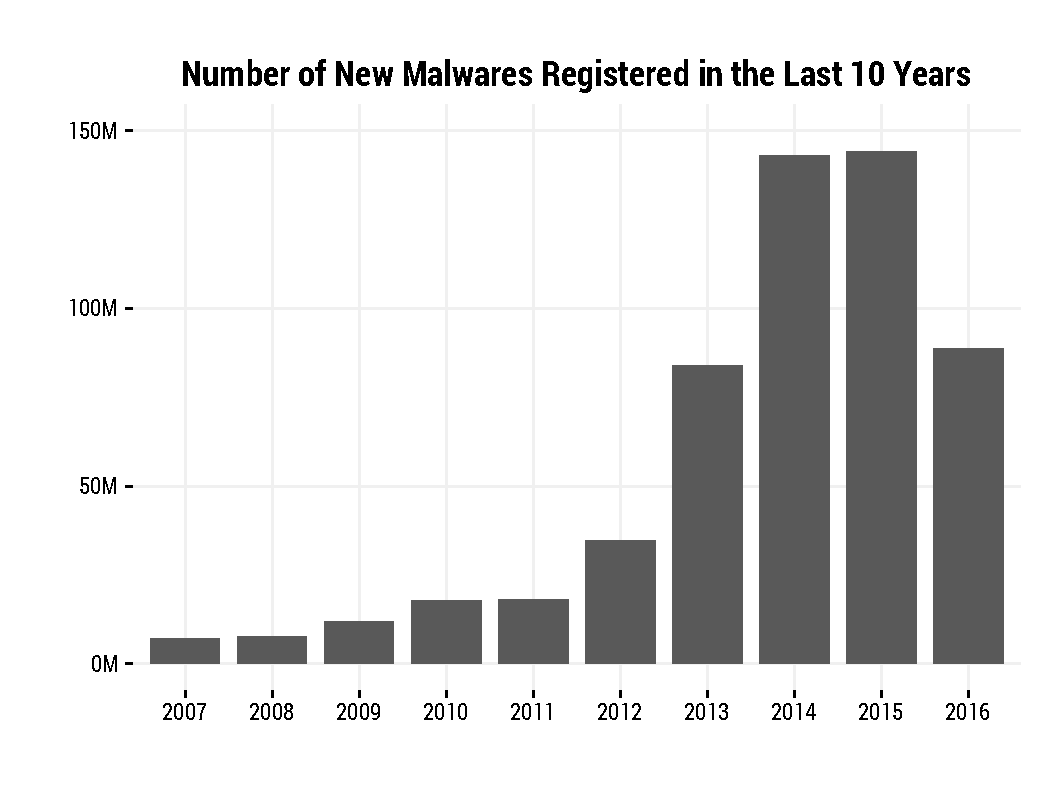
\includegraphics[width=1\linewidth]{./slideImgs/new-malware.pdf}
  \end{figure}
\end{frame}

\begin{frame}{Introduction}
  \begin{figure}
    \centering
    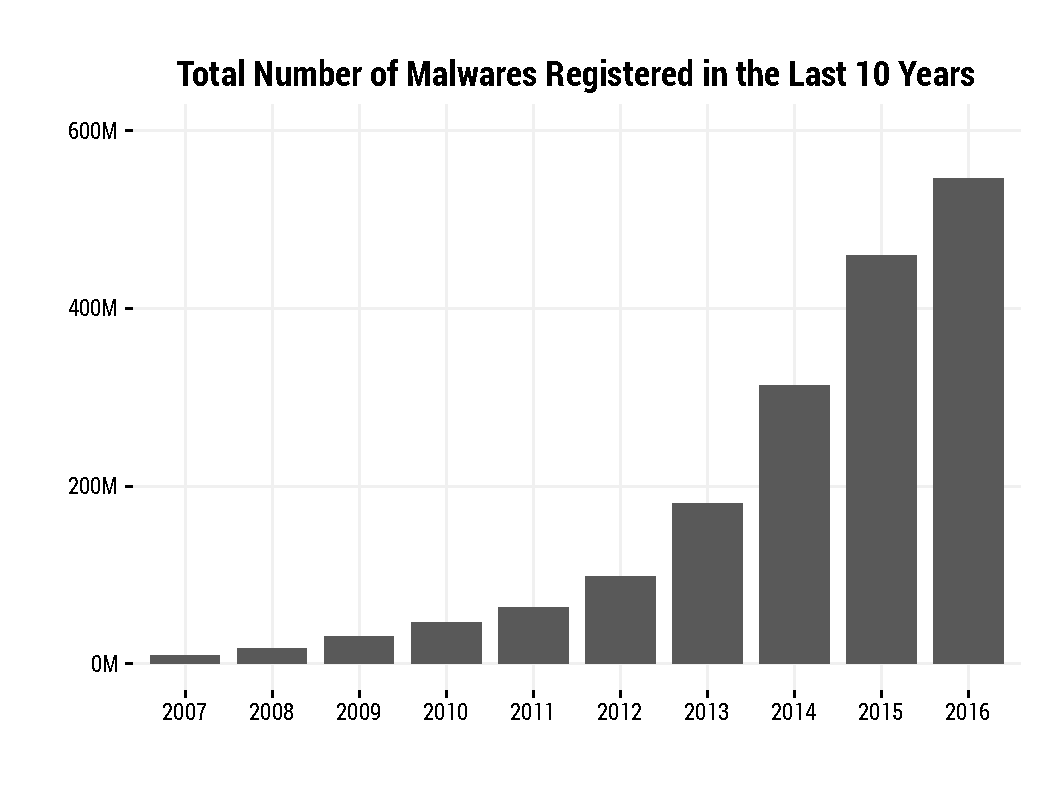
\includegraphics[width=1\linewidth]{./slideImgs/sum-malware.pdf}
  \end{figure}
\end{frame}

\begin{frame}{Introduction}
  \begin{block}{Malware Industry}
    \begin{itemize}
      \item Malware industry has become a well organized market involving large amounts of money.
      \item ``Malware as a Service''
      \begin{itemize}
        \item 400,000 Users and Organizations Globally
        \item Anyone can obtain a network controlling 10,000 compromised computers for just \$1,000.
      \end{itemize}
    \end{itemize}
  \end{block}
\end{frame}

\begin{frame}{Introduction}
  \begin{block}{Evasion}
    \begin{itemize}
      \item Since the beginning of 2015, a sizable portion of malware utilizes a combination of many techniques designed to avoid detection and analysis.
      \item Polymorphism is introduced to malwares. Malicious files belonging to the same family looks like totally different files.
      \item Malware classification has become a challenge.
    \end{itemize}
  \end{block}
\end{frame}

\begin{frame}{Goal of the Study}
  \begin{block}{Malware Classification}
    \begin{itemize}
      \item Given a malware executable, determine which family it belongs to.
      \item Build a statistical learning based framework to automatically classify malware.
    \end{itemize}
  \end{block}
\end{frame}

\begin{frame}{Background}
  \begin{block}{How are Executables Generated}
    \texttt{gcc -o helloworld helloworld.c}
    \begin{enumerate}
      \item Write code in a programming language
      \item Compiler generates assembly code version
      \item Assembler converts assembly code into binary object file
      \item Linker merges object files and libraries together and generates the executable
    \end{enumerate}
  \end{block}
\end{frame}

\begin{frame}{Background}
  \begin{block}{Representations of an Executable}
    \begin{itemize}
      \item Original code in programming language
      \item Assembly code generated by compiler
      \item Binary object file generated by assembler and linker
    \end{itemize}
  \end{block}
\end{frame}

\begin{frame}{Background}
  \begin{block}{Representations of an Executable}
    \begin{itemize}
      \item Original code in programming language {\color{red}\xmark}
      \item Assembly code generated by compiler {\color{green}\cmark}
      \item Binary object file generated by assembler and linker {\color{green}\cmark}
    \end{itemize}
  \end{block}
  Assembly and Binary code can be obtained by Interactive Disassembler (IDA)
\end{frame}

\begin{frame}[fragile]{Background}
  \begin{block}{Example of Assembly Code}
    \begin{verbatim}
    .text:00401090 8B 44 24 10    mov     eax, [esp+10h]
    .text:00401094 8B 4C 24 0C    mov     ecx, [esp+0Ch]
    .text:00401098 8B 54 24 08    mov     edx, [esp+8]
    .text:0040109C 56             push    esi
    .text:0040109D 8B 74 24 08    mov     esi, [esp+8]

    ......

    .idata:005265CC               ; Imports from WS2_32.dll
    .idata:005265CC               ;
    .idata:005265D0               ; int __stdcall WSACleanup()
    .idata:005265D0 ?? ?? ?? ??   extrn WSACleanup:dword ;
                                  CODE XREF: _WinMain@16_0+
    .idata:005265D0               ; DATA XREF: _WinMain@16_0+
    \end{verbatim}
  \end{block}
\end{frame}

\linespread{1.2}

\begin{frame}{Background}
  \begin{block}{Information in Assembly Code}
    \begin{itemize}
      \item Code segments (e.g. .text, .idata) {\color{green}\cmark}
      \item Memory address of the line of code (e.g. 00401090)
      \item Binary representation of the code (e.g. 8B 44 24 10) {\color{green}\cmark}
      \item Operation code (Opcode), single instruction executed by the CPU (e.g. mov, push) {\color{green}\cmark}
      \item Operands (e.g. eax, [esp+10h])
      \item Dynamic link libraries imported to the program (e.g. WS2\_32.dll)
      \item Function called by the program (e.g. WSACleanup)
    \end{itemize}
  \end{block}
\end{frame}

\linespread{1.3}

\begin{frame}{Dataset Description}
\begin{columns}[t]

\column{.35\textwidth}

  \begin{block}{Dataset}
    \begin{itemize}
      \item From Microsoft
      \item 10,826 malwares, all labeled
      \item 8 malware families
      \item 185 GB
      \item 2 text files for each malware variant
    \end{itemize}
  \end{block}

\column{.5\textwidth}
  \vspace*{-4ex}
  \begin{table}[ht!]
    \centering
    \caption{Malware Families}
    \begin{tabular}{lr}
      \toprule
      Family & Count\\
      \midrule
      Ramnit & 1541 \\
      Lollipop & 2478 \\
      Kelihos\_ver3 & 2942 \\
      Vundo & 475 \\
      Tracur & 751 \\
      Kelihos\_ver1 & 398 \\
      Obfuscator.ACY & 1228 \\
      Gatak & 1013 \\
      \bottomrule
    \end{tabular}
  \end{table}

\end{columns}
\end{frame}

\begin{frame}{Dataset}
  \begin{figure}
    \centering
    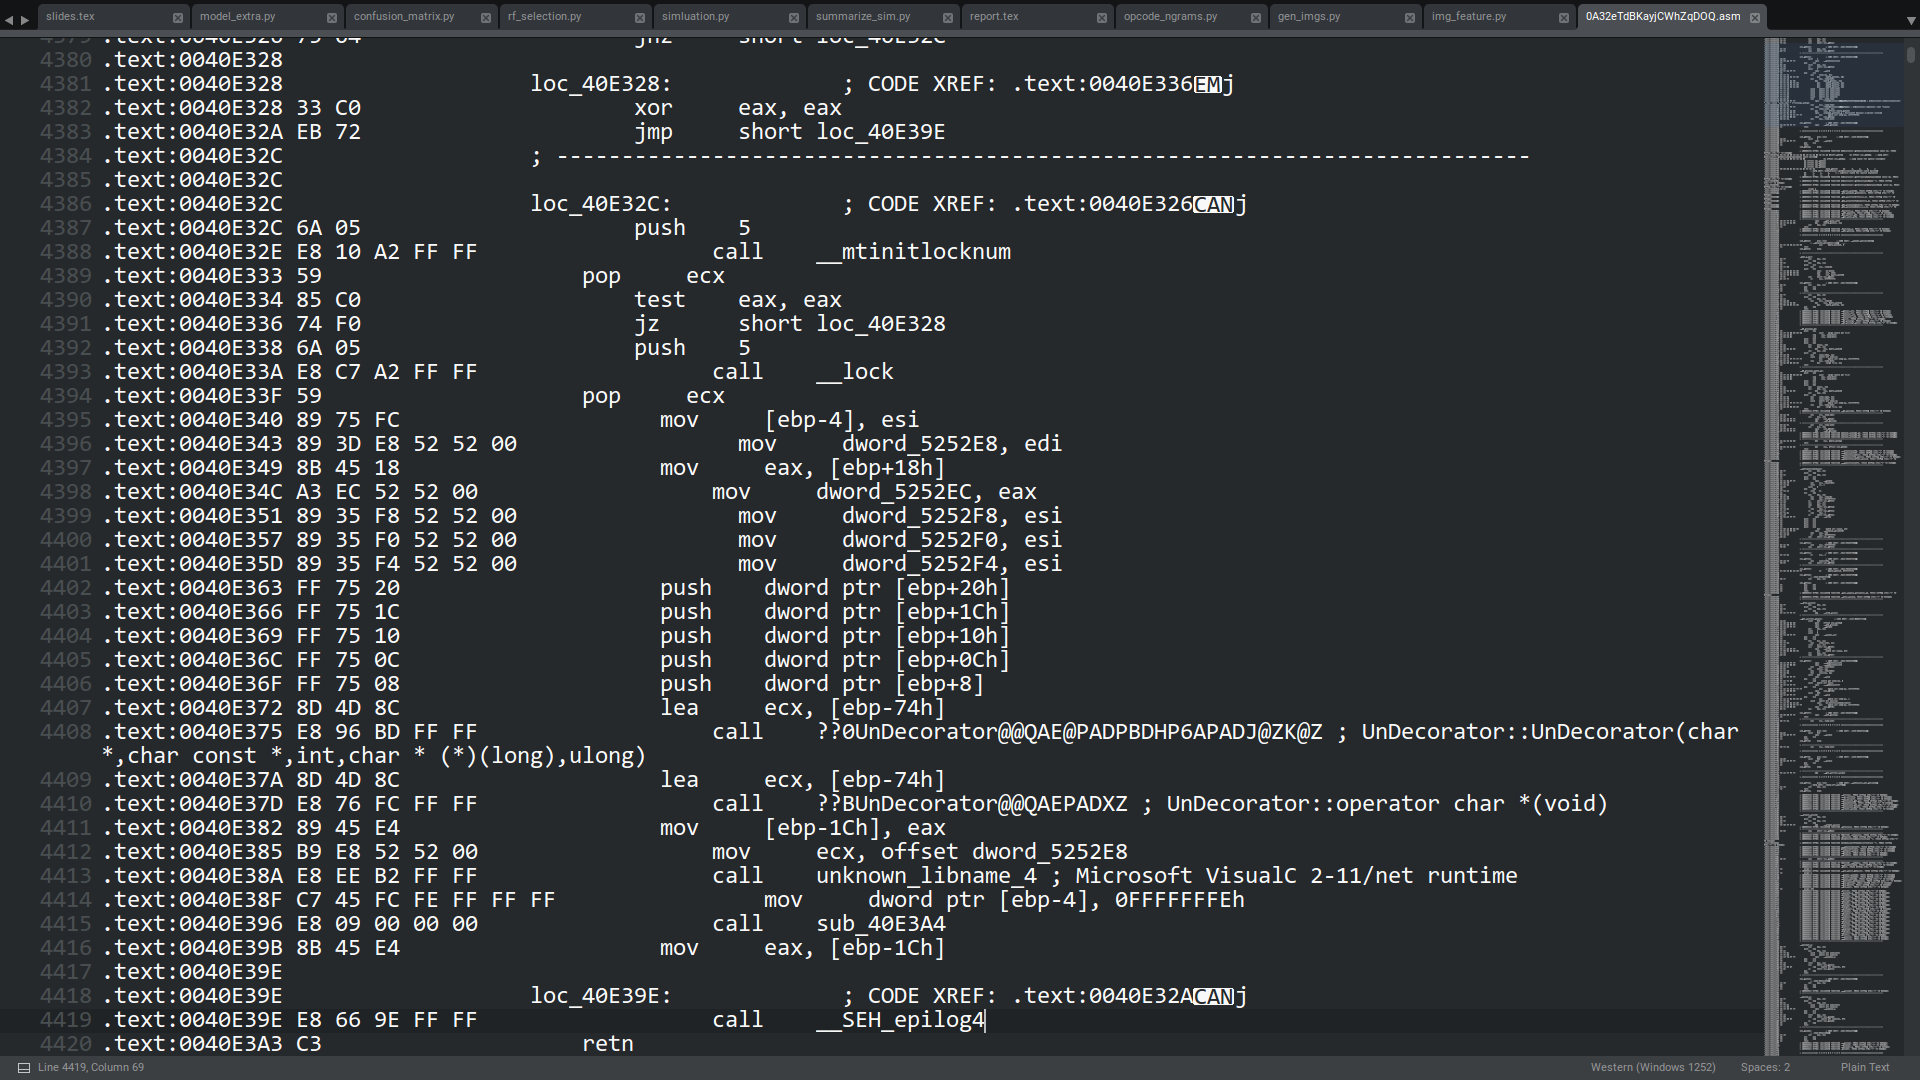
\includegraphics[width=1\linewidth]{./slideImgs/asm.png}
    \caption{.asm File}
  \end{figure}
\end{frame}


\begin{frame}{Dataset}
  \begin{figure}
    \centering
    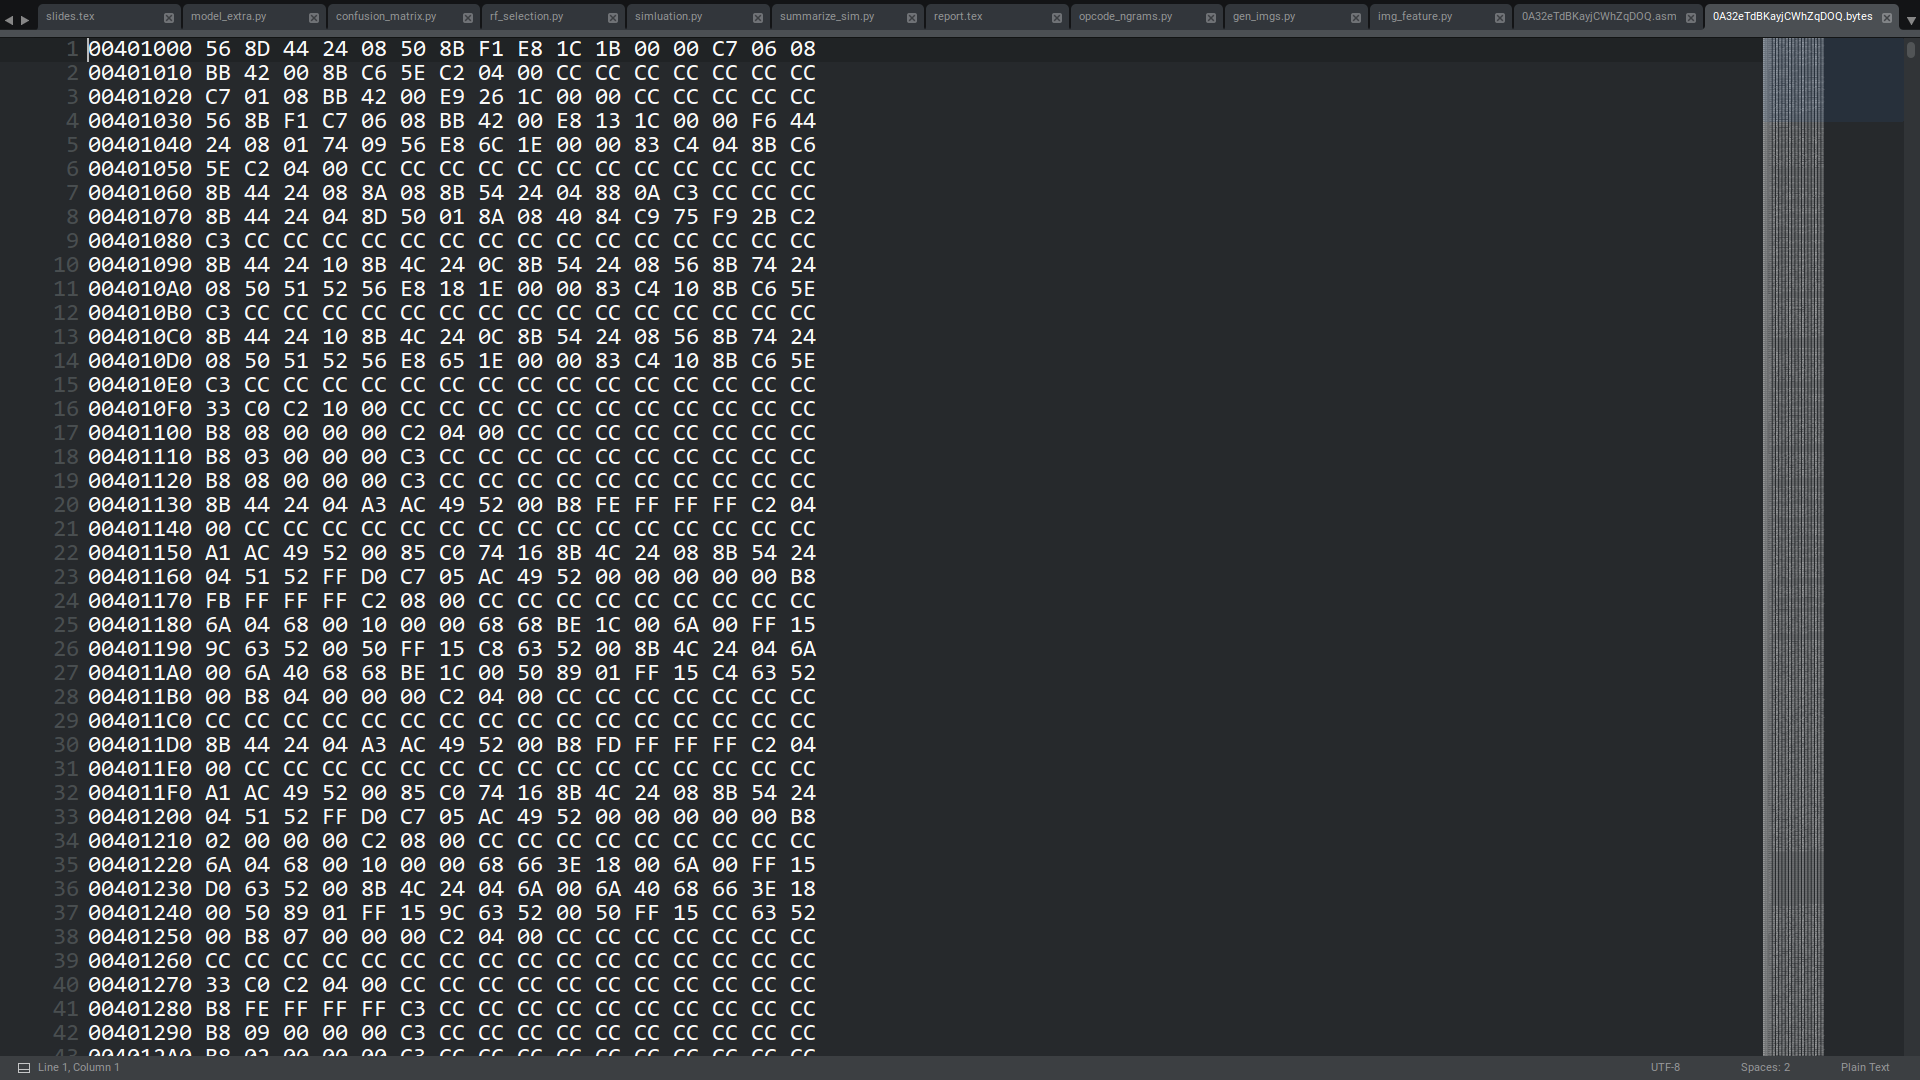
\includegraphics[width=1\linewidth]{./slideImgs/bytes.png}
    \caption{.bytes File}
  \end{figure}
\end{frame}

\begin{frame}{Feature Engineering}
  \begin{block}{Source of Features}
    \begin{itemize}
        \item Text features from ``.asm'' file
        \item Text features from ``.bytes'' file
        \item Image features from ``.bytes'' file
        \item Meta data features from both ``.asm'' file and ``.bytes'' file
    \end{itemize}
  \end{block}
\end{frame}

\begin{frame}{Feature Engineering}
  \begin{figure}[ht!]
  \centering
  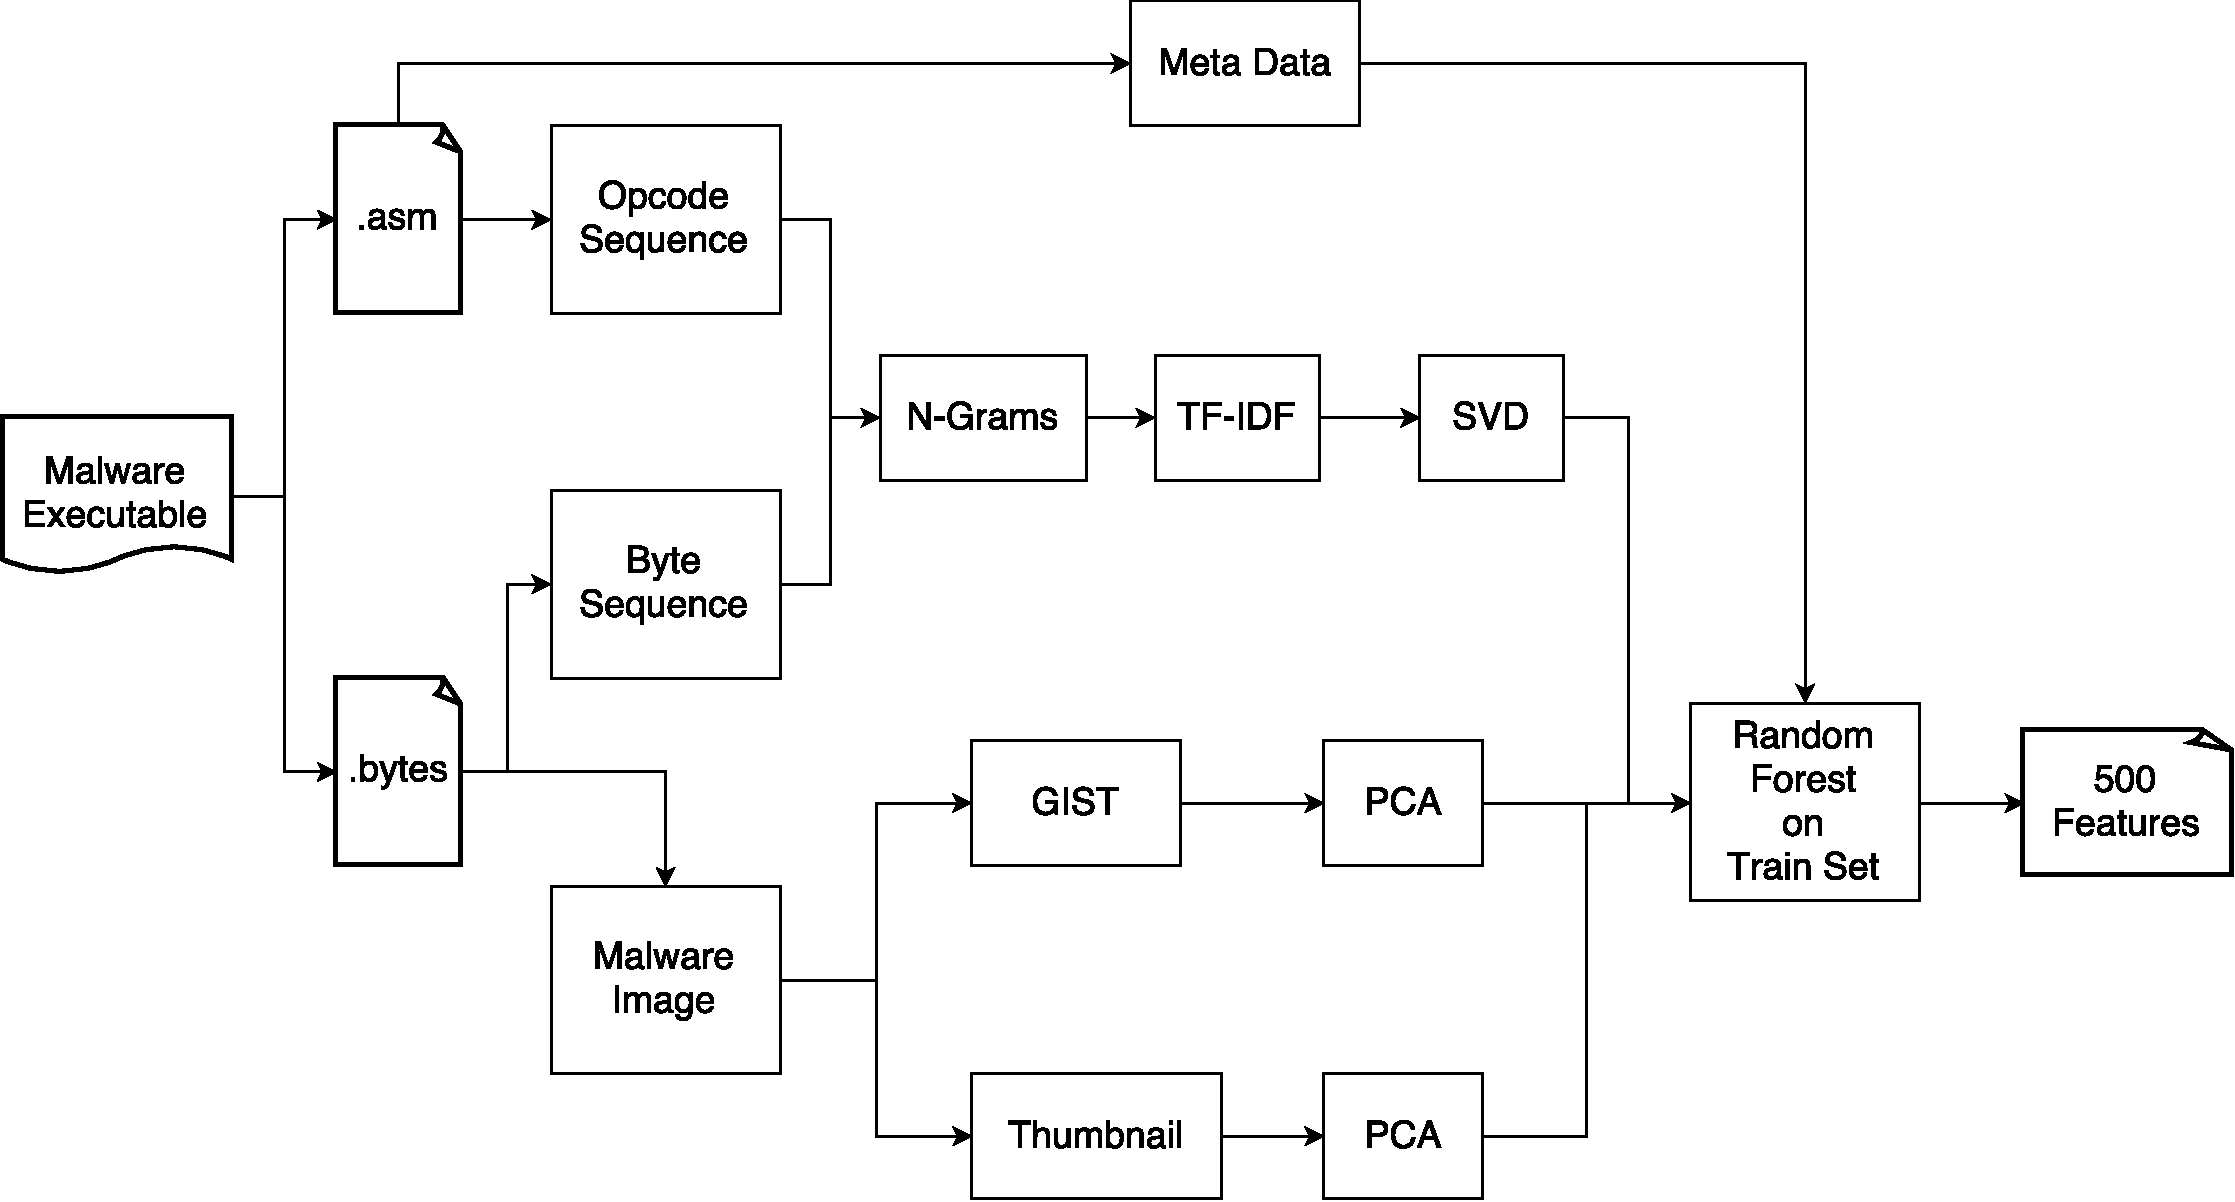
\includegraphics[width=1\linewidth]{./imgs/FeatureEngineering.pdf}
  \caption{The Feature Engineering Process}
  \end{figure}
\end{frame}

\begin{frame}{Feature Engineering}
  \begin{block}{Text Features from ``.asm'' File}
    \begin{enumerate}
      \item Extract Opcode sequence
      \item Count n-grams (n = 1, 2, 3, 4) on Opcode sequence
      \item TF-IDF to vectorize and re-weight n-grams
      \item SVD for Latent Semantic Analysis (LSA) and dimensionality reduction
    \end{enumerate}
  \end{block}
\end{frame}

\begin{frame}[fragile]{Text Features from ``.asm'' File}
  \begin{block}{Extract Opcode sequence}
    \begin{Verbatim}
    .text:00401390 8B 4C 24 04         mov     ecx, [esp+arg_0]
    .text:00401394 B8 1F CD 98 AE      mov     eax, 0AE98CD1Fh
    .text:00401399 F7 E1               mul     ecx
    .text:0040139B C1 EA 1E            shr     edx, 1Eh
    .text:0040139E 69 D2 FA C9 D6 5D   imul    edx, 5DD6C9FAh
    .text:004013A4 56                  push    esi
    .text:004013A5 57                  push    edi
    .text:004013A6 8B F9               mov     edi, ecx
    \end{Verbatim}

    Opcode Seq $\Rightarrow$ mov, mov, mul, shr, imul, push, push, mov
  \end{block}
\end{frame}

\begin{frame}[fragile]{Text Features from ``.asm'' File}
  \begin{block}{Count n-grams}
    \begin{itemize}
      \item mov, mov, mul, shr, imul, push, push, mov
      \item 1-gram $\Rightarrow$ \{mov: 3, push: 2, mul: 1, imul: 1, shr: 1\}
      \item bi-grams $\Rightarrow$ \{(mul, shr): 1, (push, push): 1, (push, mov): 1, (imul, push): 1, (mov, mul): 1, (mov, mov): 1, (shr, imul): 1\}
      \item tri-grams $\Rightarrow$ \{(shr, imul, push): 1, (mov, mov, mul): 1, (mov, mul, shr): 1, (mul, shr, imul): 1, (imul, push, push): 1, (push, push, mov): 1\}
    \end{itemize}
  \end{block}
\end{frame}

\begin{frame}{Text Features from ``.asm'' File}
  \begin{block}{n-grams}
    \begin{itemize}
        \item 658 1-gram, all
        \item 1524 bi-grams, > 150 times in at least one file
        \item 5225 tri-grams, > 100 times in at least one file
        \item 9130 4-grams, > 100 times in at least one file
    \end{itemize}
  \end{block}
\end{frame}

\begin{frame}{Text Features from ``.asm'' File}
  \begin{block}{TF-IDF}
    \begin{itemize}
      \item Let $t$ be the n-gram term, $d$ be the document, $D$ be the Corpus
      $$\mathrm{TF}(t, d) = f_{t, d} \quad \mathrm{IDF}(t, D) = \log\left(1 + \frac{N}{|\{d \in D : t \in D \}|}\right)$$
      $$\mathrm{TFIDF}(t, d, D) = \mathrm{TF}(t, d) \cdot (\mathrm{IDF}(t, D) + 1)$$
      \item Construct matrix, file as row, n-gram as column, TF-IDF as value
      \item Apply L2 normalize for each row (cosine distance)
      \item Why IDF? Tokens that occur very frequently in a given corpus are not informative
  \end{itemize}
  \end{block}
\end{frame}

\begin{frame}{Text Features from ``.asm'' File}
  \begin{block}{SVD}
    \begin{itemize}
      \item Latent Semantic Analysis and Dimensionality Reduction
      \item $M_{m, n} = U_{m, m} \Sigma_{m, n} V^{T}_{n, n}$
      \item $M_{m, n} \approx U_{m, k} \Sigma_{k, k} V^{T}_{n, k}$ closest approximation with rank k
      \item $U_{m, k}$ the reduced version of $M$, with $k$ Topic vectors
      \item Choose $k$, use theorem
      $$||M||_{F}^{2} = \sum \sigma_{i}^{2}$$
      \item 95\% norm explained is fine
    \end{itemize}
  \end{block}
\end{frame}

\begin{frame}
  \begin{block}{SVD}
    \begin{itemize}
        \item 100 1-gram topics
        \item 200 2-gram topics
        \item 400 3-gram topics
        \item 500 4-gram topics
        \item Total from 16537 to 1200
    \end{itemize}
  \end{block}
\end{frame}

\begin{frame}{Feature Engineering}
  \begin{block}{Text Features from ``.bytes'' File}
    \begin{enumerate}
      \item Extract Byte sequence
      \item Count n-grams (n = 1, 2, 4) on Byte sequence
      \item TF-IDF to vectorize and re-weight n-grams
      \item SVD for Latent Semantic Analysis (LSA) and dimensionality reduction
    \end{enumerate}
  \end{block}
\end{frame}

\begin{frame}{Feature Engineering}
  \begin{block}{Image Features From ``.bytes'' File}
    \begin{enumerate}
      \item Visualize malware image and scale it
      \item Obtain feature vector by GIST descriptor and PCA
      \item Obtain feature vector by image thumbnail and PCA
    \end{enumerate}
  \end{block}
\end{frame}

\begin{frame}{Image Features From ``.bytes'' File}
  \begin{block}{Malware Visualization}
    \begin{itemize}
      \item From .bytes file, instructions are represented sequence of double hexadecimal points
      \item 00 to FF in hex is 0 to 255
      \item Use this value as a gray scale value
      \item Determine the width of image
    \end{itemize}
  \end{block}
\end{frame}

\begin{frame}{Image Features From ``.bytes'' File}
\begin{figure}[ht!]
\begin{subfigure}{.45\textwidth}
  \centering
  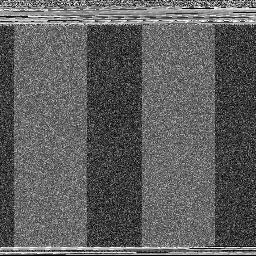
\includegraphics[width=.45\linewidth]{./imgs/MalwareSample/2/01IsoiSMh5gxyDYTl4CB.jpg}
  \caption{01IsoiSMh5gxyDYTl4CB}
\end{subfigure}%
\begin{subfigure}{.45\textwidth}
  \centering
  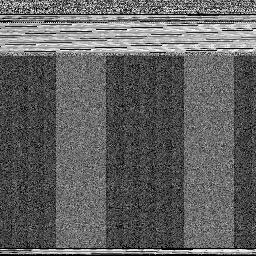
\includegraphics[width=.45\linewidth]{./imgs/MalwareSample/2/02zcUmKV16Lya5xqnPGB.jpg}
  \caption{02zcUmKV16Lya5xqnPGB}
\end{subfigure}
\begin{subfigure}{.45\textwidth}
  \centering
  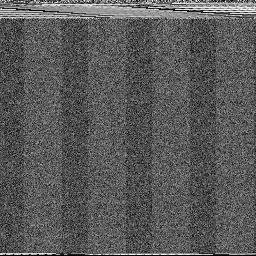
\includegraphics[width=.45\linewidth]{./imgs/MalwareSample/2/2ZNUOyAMv67lcYPoetkR.jpg}
  \caption{2ZNUOyAMv67lcYPoetkR}
\end{subfigure}
\begin{subfigure}{.45\textwidth}
  \centering
  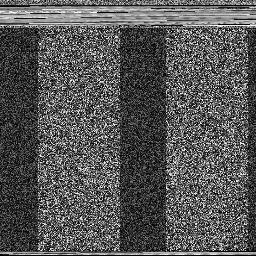
\includegraphics[width=.45\linewidth]{./imgs/MalwareSample/2/40ofYnDCl8TKJXwyGmrP.jpg}
  \caption{40ofYnDCl8TKJXwyGmrP}
\end{subfigure}
\caption{Sample Malware Images for Lollipop}
\label{malware image lollipop}
\end{figure}
\end{frame}

\begin{frame}{Image Features From ``.bytes'' File}
\begin{figure}[ht!]
\begin{subfigure}{.45\textwidth}
  \centering
  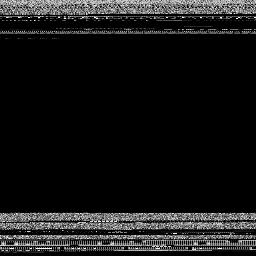
\includegraphics[width=.45\linewidth]{./imgs/MalwareSample/8/0AguvpOCcaf2myVDYFGb.jpg}
  \caption{0AguvpOCcaf2myVDYFGb}
\end{subfigure}%
\begin{subfigure}{.45\textwidth}
  \centering
  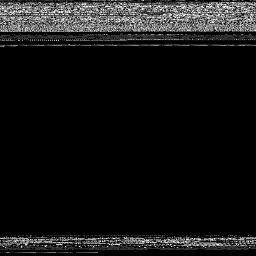
\includegraphics[width=.45\linewidth]{./imgs/MalwareSample/8/2TaBCxc4msyVU5YDRuOd.jpg}
  \caption{2TaBCxc4msyVU45YDRuOd}
\end{subfigure}
\begin{subfigure}{.45\textwidth}
  \centering
  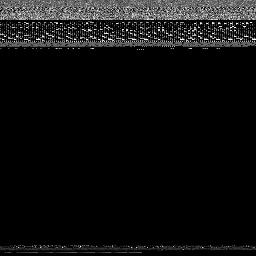
\includegraphics[width=.45\linewidth]{./imgs/MalwareSample/8/6jCs7bHULZXW3kKtxNRw.jpg}
  \caption{6jCs7bHULZXW3kKtxNRw}
\end{subfigure}
\begin{subfigure}{.45\textwidth}
  \centering
  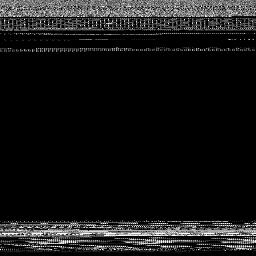
\includegraphics[width=.45\linewidth]{./imgs/MalwareSample/8/8lTjbp3rnwtLh104E57v.jpg}
  \caption{8lTjbp3rnwtLh104E57v}
\end{subfigure}
\caption{Sample Malware Images for Obfuscator.ACY}
\label{malware image Obfuscator}
\end{figure}
\end{frame}

\begin{frame}{Image Features From ``.bytes'' File}
\begin{figure}[ht!]
\begin{subfigure}{.45\textwidth}
  \centering
  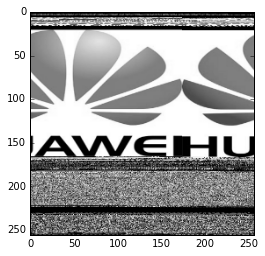
\includegraphics[width=.55\linewidth]{./slideImgs/fun1.png}
  \caption{5764RnJYTirWq1utgdkN}
\end{subfigure}%
\begin{subfigure}{.45\textwidth}
  \centering
  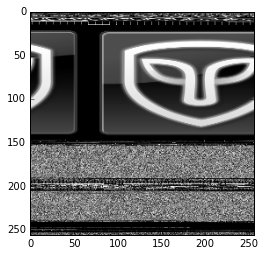
\includegraphics[width=.55\linewidth]{./slideImgs/fun2.png}
  \caption{2DBKbxPnVCyiLzqAHU9c}
\end{subfigure}
\begin{subfigure}{.45\textwidth}
  \centering
  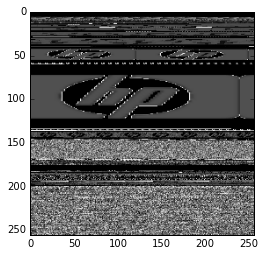
\includegraphics[width=.55\linewidth]{./slideImgs/fun3.png}
  \caption{NxrC3kQvsl5AZ4WtowHD}
\end{subfigure}
\begin{subfigure}{.45\textwidth}
  \centering
  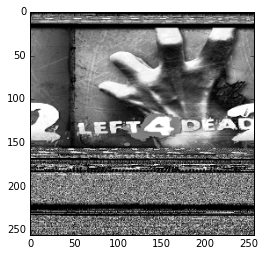
\includegraphics[width=.55\linewidth]{./slideImgs/fun4.png}
  \caption{goYPdUatw3BQEl6iCI0D}
\end{subfigure}
\caption{Fun Malware Image}
\label{fun}
\end{figure}
\end{frame}

\begin{frame}{Image Features From ``.bytes'' File}
  \begin{block}{GIST}
    \begin{itemize}
      \item Convolve the image with 20 pre-designed Gabor filters to construct 20 feature maps
      \item Divide each feature map into 16 regions (by a $4 \times 4$ grid)
      \item Average the feature values within each region
      \item Concatenate feature values together, length 320
      \item PCA for dimension reduction
    \end{itemize}
  \end{block}
\end{frame}

\begin{frame}{Image Features From ``.bytes'' File}
\begin{figure}[ht!]
\centering
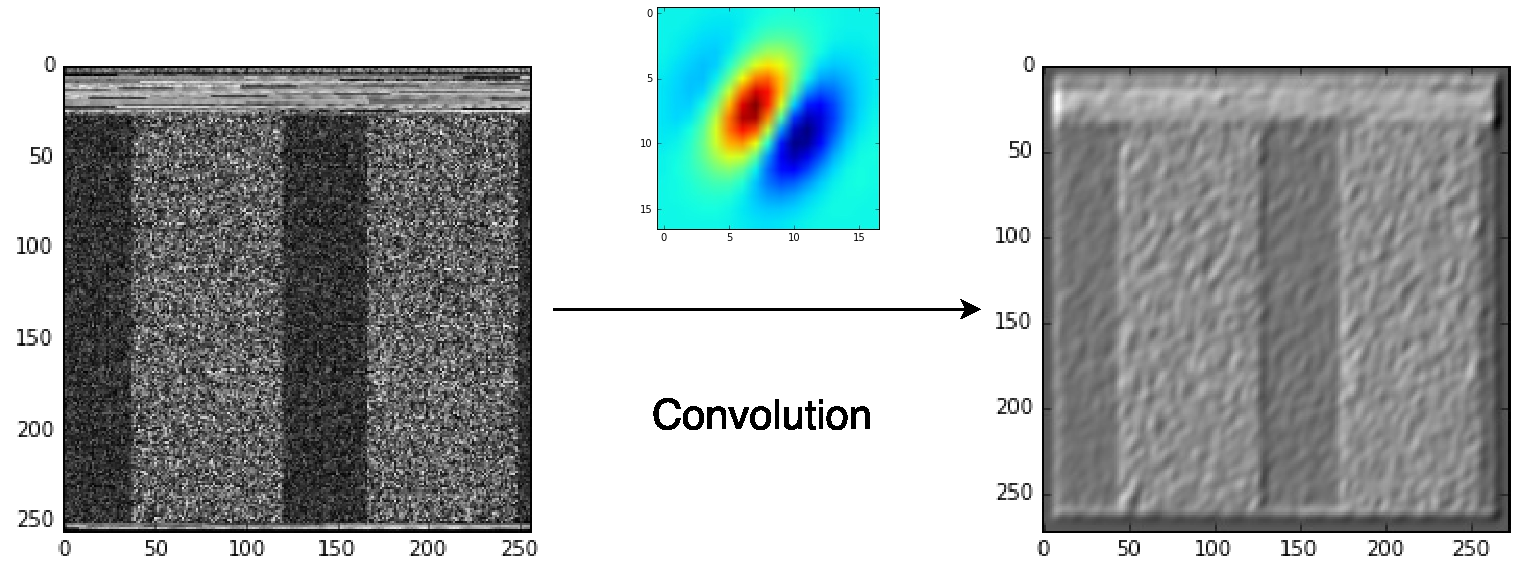
\includegraphics[width=1\linewidth]{./slideImgs/gist.pdf}
\caption{GIST}
\label{gist}
\end{figure}
\end{frame}

\begin{frame}{Image Features From ``.bytes'' File}
  \begin{block}{Image Thumbnail}
    \begin{itemize}
      \item Rescale the image to $32 \times 32$ and flatten it to a vector
      \item PCA for dimension reduction
    \end{itemize}
  \end{block}
\end{frame}

\begin{frame}{Feature Engineering}
  \begin{block}{Meta Data Features From Both ``.asm'' File and ``.bytes'' File}
    \begin{itemize}
      \item Segment count from ``.asm'' file (.text, .data, .idata), TF-IDF, SVD
      \item File size for ``.asm'' file
      \item File size for ``.bytes'' file
    \end{itemize}
  \end{block}
\end{frame}

\begin{frame}{Feature Engineering}
  \begin{block}{Concatenation and Selection}
    \begin{itemize}
      \item Concatenate all features together, more than 4,000
      \item Supervised feature selection by training Random Forest on the Training Set, 500 ultimate features
    \end{itemize}
  \end{block}
\end{frame}

\begin{frame}{Feature Engineering}
\begin{figure}[ht!]
\centering
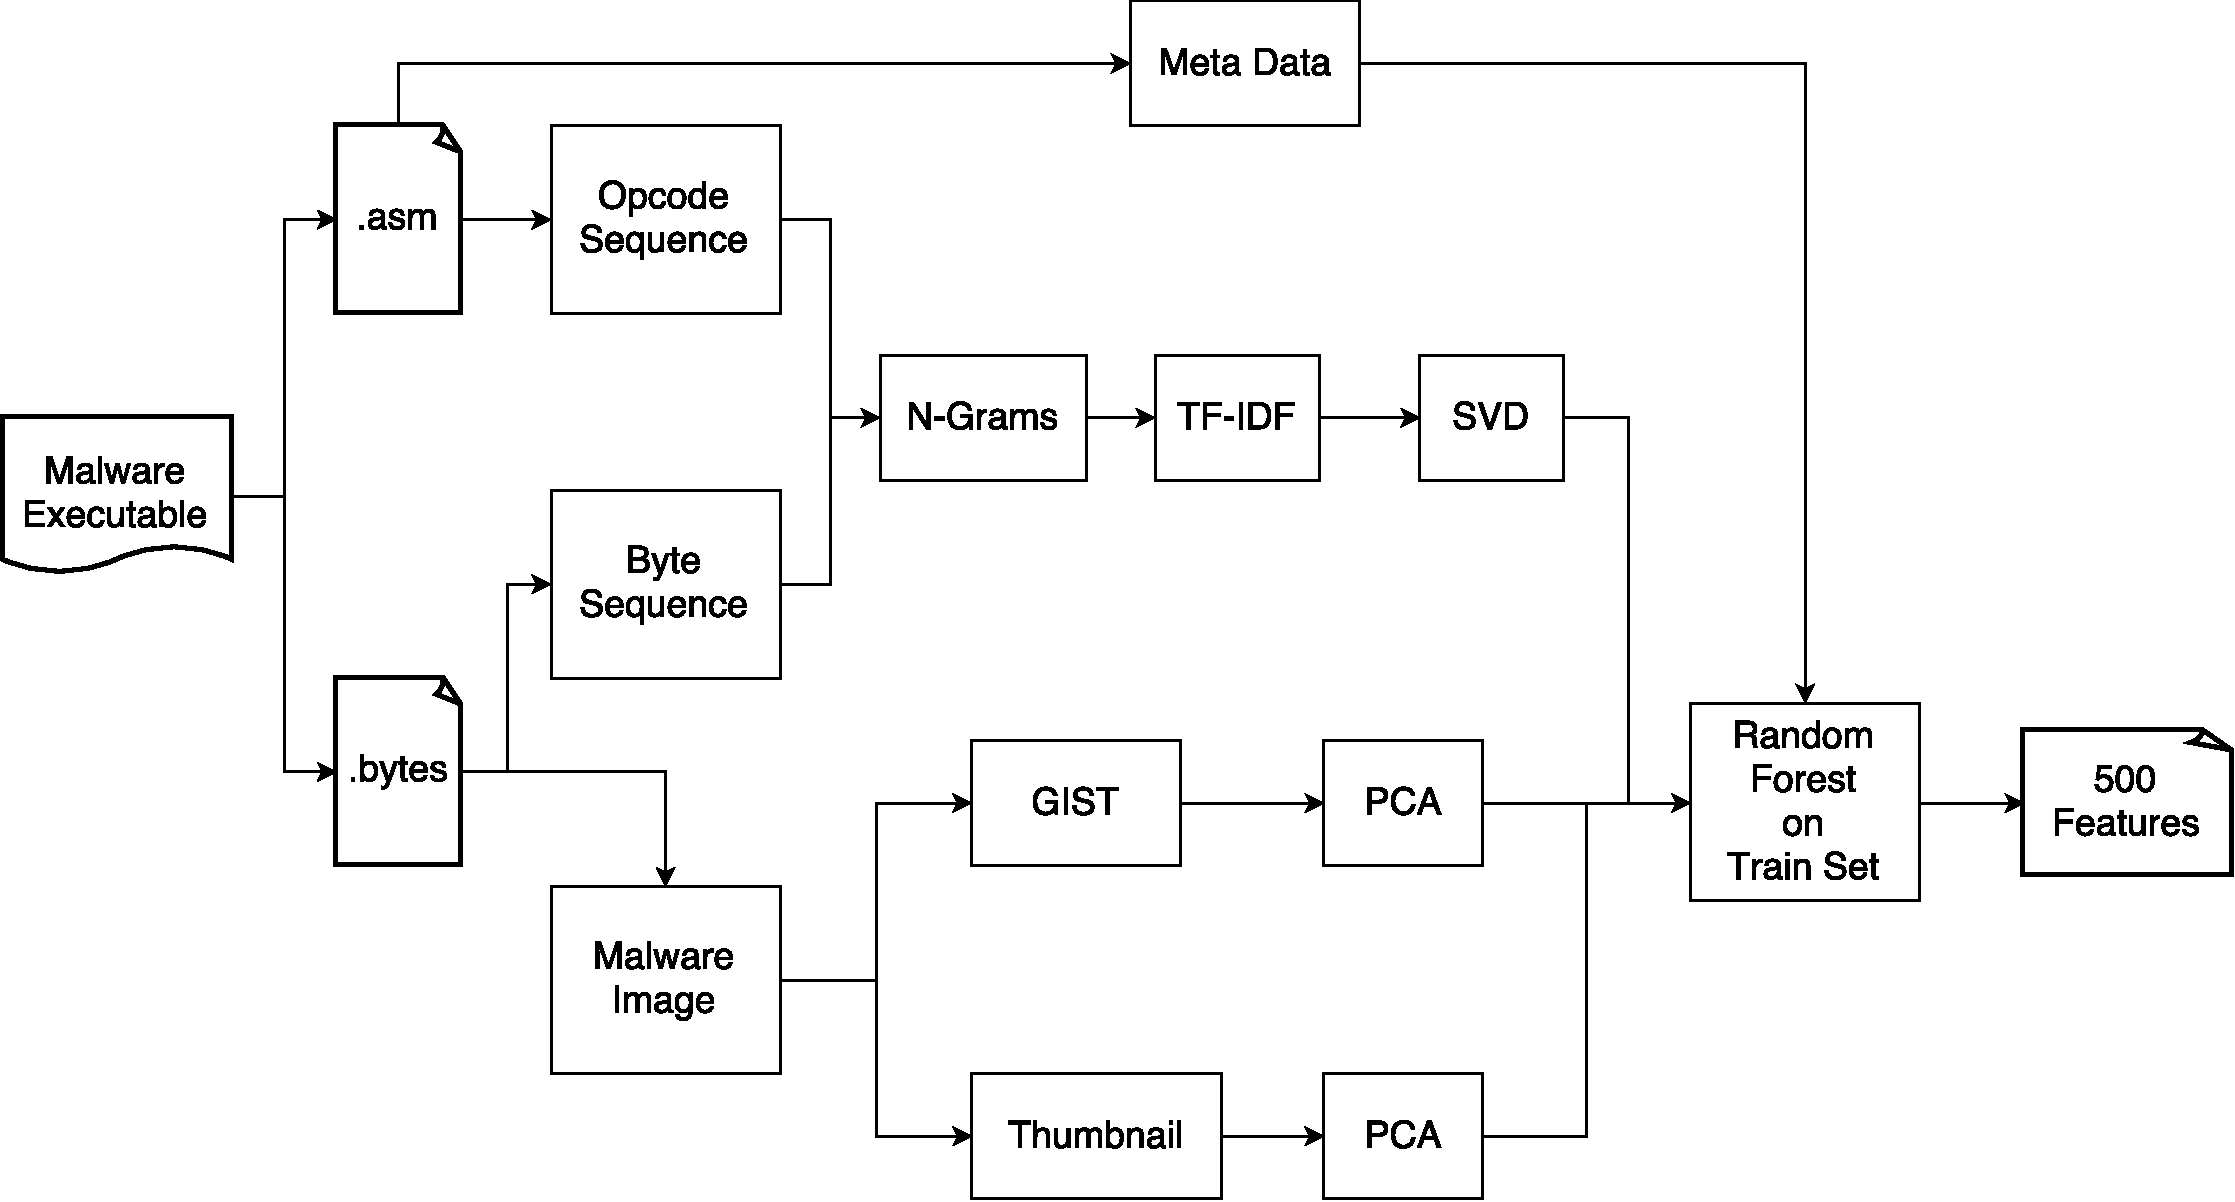
\includegraphics[width=1\linewidth]{./imgs/FeatureEngineering.pdf}
\caption{The Feature Engineering Process}
\end{figure}
\end{frame}

\begin{frame}{Feature Engineering}
\begin{figure}[htbp]
\centering
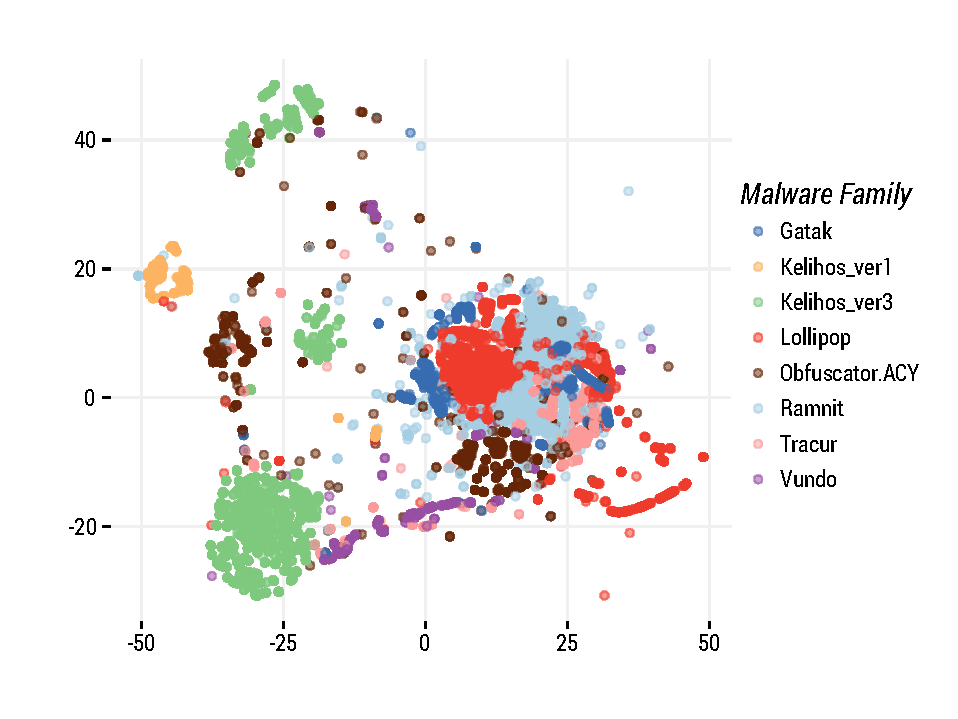
\includegraphics[width=.9\linewidth]{./imgs/tsne.pdf}
\caption{t-SNE Visualization with 500 Selected Features}
\label{t-sne}
\end{figure}
\end{frame}

\begin{frame}{Predictive Modeling}
  \begin{block}{Candidates}
    \begin{itemize}
      \item Generative Model
      \begin{itemize}
        \item Naive Bayes (NB)
        \item Linear Discriminant Analysis (LDA)
        \item Quadratic Discriminant Analysis (QDA)
      \end{itemize}
      \item Discriminative model
      \begin{itemize}
        \item Multinomial Logistic Regression (Multi-Logreg)
        \item One-vs-Rest Logistic Regression (OvR-Logreg)
        \item Support Vector Machine with Probability Calibration (SVM)
        \item Random Forest Classifier (RF)
        \item Extremely randomized trees (ExtraTrees)
        \item eXtreme Gradient Boosting (XGBoost)
      \end{itemize}
    \end{itemize}
  \end{block}
\end{frame}

\begin{frame}{Generative Model}
  \begin{block}{Idea}
    \begin{itemize}
      \item Estimate $P(\vec{x} | y)$ based on different assumptions
      \item Make prediction by Bayes' Rule
      $$P(y|\vec{x}) = \frac{P(\vec{x}|y)p(y)}{P(\vec{x})}$$
    \end{itemize}
  \end{block}
\end{frame}

\begin{frame}{Generative Model}
  \begin{block}{Candidates}
    \begin{itemize}
      \item NB, independent Gaussian: $P(\vec{x} | y) = P(x_{1}|y)P(x_{2}|y)\dots$
      \item LDA, Multi-Gaussian, same Covariance Matrix across classes
      \item QDA, Multi-Gaussian, different Covariance Matrix
    \end{itemize}
  \end{block}
\end{frame}

\begin{frame}{Discriminative Model}
  \begin{block}{Idea}
    \begin{itemize}
      \item Directly model $P(y | \vec{x})$
      \item Training by Maximum a Posteriori, or Maximum Likelihood
    \end{itemize}
  \end{block}
\end{frame}

\begin{frame}{Discriminative Model}
  \begin{block}{Logistic Regression}
    \begin{itemize}
      \item Linear combination of features
      \item Softmax function
      \item Minimize cross entropy with one-hot encoding
      \item Multinomial and One-vs-Rest
    \end{itemize}
  \end{block}
\end{frame}

\begin{frame}{Discriminative Model}
  \begin{block}{Support Vector Machine}
    \begin{itemize}
      \item Primal form
      $$ \min_{w, b} {\frac {1}{n}}\sum _{i=1}^{n}\zeta _{i}+\lambda ||w||^{2} \quad \text{s.t}. \quad y_{i}(x_{i}\cdot w+b)\geq 1-\zeta _{i}\,{\text{ and }}\,\zeta _{i}\geq 0$$
      \item Dual form
      \begin{equation*}
      \begin{split}
      \max_{a_{1}, \dots, a_{n}} f(a_{1}\ldots a_{n})=\sum _{i=1}^{n}a_{i}-{\frac {1}{2}}\sum _{i=1}^{n}\sum _{j=1}^{n}y_{i}a_{i}(x_{i}\cdot x_{j})y_{j}a_{j}\\
      \text{s.t}. \quad \sum _{i=1}^{n}a_{i}y_{i}=0,\,{\text{and }}0\leq a_{i}\leq {\frac {1}{2n\lambda }}
      \end{split}
      \end{equation*}
    \end{itemize}
  \end{block}
\end{frame}

\begin{frame}{Discriminative Model}
  \begin{block}{Support Vector Machine}
    \begin{itemize}
      \item Kernel tricks for non-linear classification (Gaussian kernel)
      \item Probability calibration: Bining or softmax fitting
     \end{itemize}
  \end{block}
\end{frame}

\begin{frame}{Discriminative Model}
  \begin{block}{Random Forest}
    \begin{itemize}
      \item Ensemble of classification trees
      \item Bootstrap sampling
      \item Randomly select features for each node split
    \end{itemize}
  \end{block}
  \begin{block}{Extremely Randomized Trees}
    \begin{itemize}
      \item Randomly draw threshold for each node split
    \end{itemize}
  \end{block}
\end{frame}

\begin{frame}{Discriminative Model}
  \begin{block}{eXtreme Gradient Boosting}
    \begin{itemize}
      \item Minimize a loss function (Logloss in this case)
      \item Additively minimize the loss function by adding classification trees
      \item The first and second order information is used in building each classification tree
    \end{itemize}
  \end{block}
\end{frame}

\begin{frame}{Evaluation}
  \begin{block}{Data Split}
    \begin{itemize}
      \item 5\% train set (542), 95\% test set (10,248) by randomized stratified sampling.
      \item Enlarge the difference among classifiers
      \item More stable estimation of predictive metrics
      \item Cross-validation for hyper-parameter tunning
      \item Repeat the procedure for 10 times
    \end{itemize}
  \end{block}
\end{frame}

\begin{frame}{Evaluation}
  \begin{block}{Metrics}
    \begin{itemize}
      \item Multi-class Logloss
      $$\mathrm{Logloss} = -\frac{1}{N}\sum_{i = 1}^{N}\sum_{j = 1}^{M}y_{ij} \log(p_{ij})$$
      \item Multi-class Accuracy
      $$\mathrm{Accuracy = 1 - \frac{\# \mathrm{misclassified}}{N}}$$
    \end{itemize}
  \end{block}
\end{frame}

\begin{frame}{Evaluation}
  \begin{block}{Metrics}
    \begin{itemize}
      \item Recall, Precision and $F_{1}$ score for each malware family
      $$\mathrm{Recall} = \mathrm{TPR} = \frac{\mathrm{TP}}{\mathrm{TP} + \mathrm{FN}}$$
      $$\mathrm{Precision} = 1 - \mathrm{FDR} = \frac{\mathrm{TP}}{\mathrm{TP} + \mathrm{FP}}$$
      $$F_{1} = 2 \cdot \frac{\mathrm{Precision} \cdot \mathrm{Recall}}{\mathrm{Precision} + \mathrm{Recall}}$$
    \end{itemize}
  \end{block}
\end{frame}

\begin{frame}{Result}
\begin{figure}[p!]
\centering
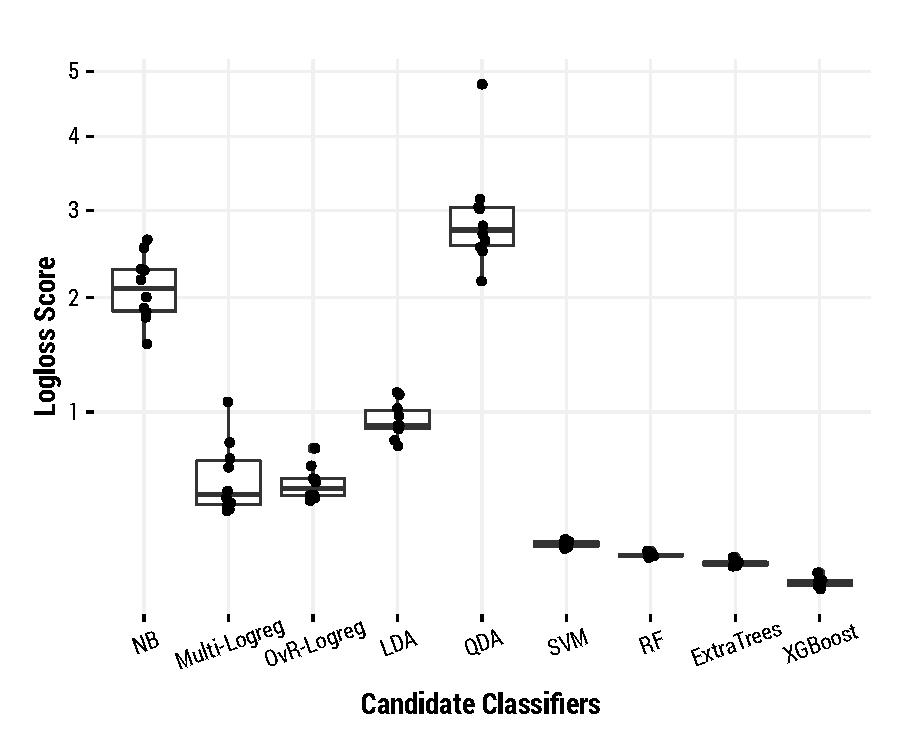
\includegraphics[width=.8\linewidth]{./imgs/logloss.pdf}
\caption{Model Evaluation: Multi-Class Logloss}
\label{logloss}
\end{figure}
\end{frame}

\begin{frame}{Result}
\begin{figure}[p!]
\centering
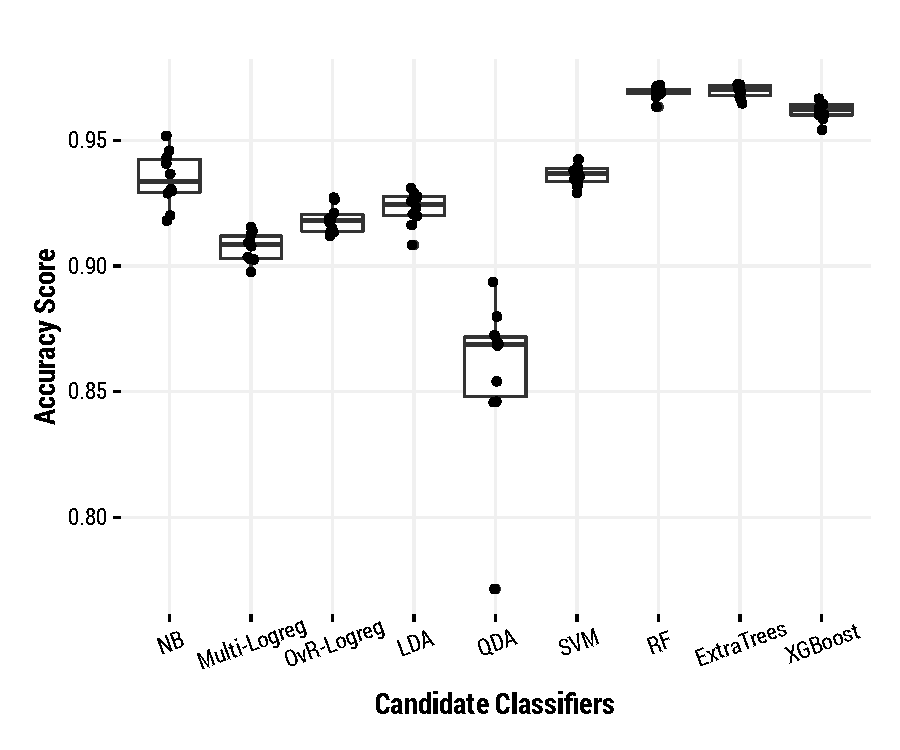
\includegraphics[width=.8\linewidth]{./imgs/acc.pdf}
\caption{Model Evaluation: Multi-Class Accuracy}
\label{acc}
\end{figure}
\end{frame}

\begin{frame}{Result}
\begin{table}[ht!]
\centering
\caption{Confusion Matrix for Extremely Randomized Trees}
\begin{tabular}{cccccccc}
\toprule
 $1422$ & $28$ & $0$ & $0$ & $0$ & $0$ & $14$ & $0$ \\
 $24$ & $2329$ & $0$ & $0$ & $1$ & $0$ & $0$ & $0$ \\
 $0$ & $9$ & $2785$ & $0$ & $1$ & $0$ & $0$ & $0$ \\
 $3$ & $24$ & $0$ & $414$ & $2$ & $0$ & $6$ & $2$ \\
 $7$ & $32$ & $0$ & $2$ & $671$ & $0$ & $1$ & $0$ \\
 $4$ & $8$ & $0$ & $0$ & $0$ & $364$ & $2$ & $0$ \\
 $80$ & $16$ & $0$ & $2$ & $4$ & $0$ & $1065$ & $0$ \\
 $2$ & $6$ & $0$ & $0$ & $2$ & $0$ & $12$ & $940$ \\
\bottomrule
\end{tabular}
\end{table}
\end{frame}

\begin{frame}{Result}
  \begin{table}[ht!]
    \centering
    \caption{Classification Report for Extremely Randomized Trees}
    \begin{tabular}{lrrrr}
      \toprule
      Family & Rrecision & Recall & $F_{1}$ Score & Support \\
      \midrule
      Ramnit        &       0.92&      0.97&      0.94&      1464\\
      Lollipop      &       0.96&      0.99&      0.97&      2354\\
      Kelihos\_ver3 &       1.00&      1.00&      1.00&      2795\\
      Vundo         &       0.99&      0.92&      0.95&       451\\
      Tracur        &       0.99&      0.94&      0.96&       713\\
      Kelihos\_ver1 &       1.00&      0.96&      0.98&       378\\
      Obfuscator.ACY&       0.96&      0.91&      0.93&      1167\\
      Gatak         &       1.00&      0.98&      0.99&       962\\
      \midrule
      Avg / Total   &       0.97&      0.97&      0.97&      10284\\
      \bottomrule
    \end{tabular}
  \end{table}
\end{frame}


\begin{frame}
  \begin{table}[p]
  \centering
  \begin{tabular}{c}
  \Huge Question?
  \end{tabular}
  \end{table}
\end{frame}

\begin{frame}
  \begin{table}[p]
  \centering
  \begin{tabular}{c}
  \Huge Thank You!
  \end{tabular}
  \end{table}
\end{frame}



\end{document}

